%!TEX root = proposal.tex


\section{ORDINARY KRIGING FOR SPATIALLY INDEXED FUNCTIONAL DATA}
\label{functional kriging}
%\begin{spacing}{1.9}

\subsection{Introduction}


Data that arise from environmental processes often exhibit similarities at small spatial scales. Geostatistical models incorporate this phenomenon by  modeling correlations as a function of distance. Often a primary goal of the analysis is prediction of a environmental variable at an unobserved location. In this setting, geostatistical models are particularly useful because the spatial process is considered to be a continuous stochastic process. The extension of geostatistical models for functional data were first considered in \cite{Goulard:1993} where two approaches are proposed:  one approach involves cokriging by reducing the functional response to a multivariate response, while the other approach utilizes a functional version of the variogram.  The functional variogram approach has been further developed by \cite{Giraldo:2010jx} and \cite{Nerini:2010ba}. We pursue the first option, but do not make the assumption of a parametric model for the curves. We allow the curves to be represented nonparametrically using a principal component function basis. Typically, very few principal component functions are needed to represent the major modes of variation in the curves, thus making a multivariate geostatistical approach feasible. 

%==================================================
\subsection{Statistical model for spatially indexed functional data}

%Geostatics for scalar valued random fields:
%\[
%	 \left\{ \boldsymbol\chi_s: s \in D  \subseteq \Real^2\right\} 
%\] 
%data: $\left\{ \chi_{s_1}, \chi_{s_2}, \dots, \chi_{s_n} \right\} \hspace{0.2cm} i = 1, \dots, n$
%
%Kriging predictor (Best linear unbiased predictor):
%
%\[
%\widehat{\chi_{s_0}} = \sum_{i=1}^n \lambda_i \chi_{s_i}
%\]
%Unbiased constraint: 
%\[
%\sum_{i=1}^n \lambda_i = 1
%\]
%Weights $\lambda_i$ are determined by the variogram
%\[
%\gamma(h) = \frac{1}{2}Var(\chi_{s+h} -\chi_s)
%\]
In order to extend the methodology for spatial random fields to the functional setting we define a \emph{spatial functional process} as 
	\[
	 \left\{ \boldsymbol\chi(s; t): s \in D  \subseteq \Real^2, t \in \T \right\},
	 \] 
	 
	where, for fixed location $s$, $\boldsymbol\chi(s; \cdot)$ is a random function on a compact set $\mathcal{T} \subset \Real$. We assume $\boldsymbol\chi(s; \cdot)$  takes values in a reproducing kernel Hilbert space of functions $\H$. \\[0.2cm]
	
	The trajectories $\chi(s;t)$ admit the following representation 
\begin{equation}
 	\chi(s;t) = \mu(t) + \epsilon(s;t),
\end{equation}
where $\mu(t)$ represents large-scale structure which does not depend on spatial location and $\epsilon(s;t)$ is a mean zero spatially correlated random effect. The methodology we propose assumes $\epsilon(s;t)$ can be represented by the Karhunen-Loeve expansion $\epsilon(s;t) = \sum_{k=1}^{\infty} \alpha_k(s)\psi_k(t)$. The functions $\psi_k(\cdot)$ are eigenfuncitons of the covariance function and form a basis for $\L_2(\T)$. For each integer $k$, $\alpha_k(s) = \inner{\epsilon(s;t)}{ \psi_k(t)}$ is assumed to be a second-order stationary isotropic random field. Spatial random fields connected to different eigenfunctions are assumed to be uncorrelated, that is 
\begin{equation}
	\text{Cov}(\alpha_j(s), \alpha_l(s')) = 0 \hspace{1cm} \text{for } j \neq l.
	\label{eq:nocrosscor}
\end{equation} 

Under assumption  \eqref{eq:nocrosscor}, the covariance between trajectories at locations $s_j$ and $s_l$ are given by 
\begin{align}
	\text{Cov}(\chi(s_j,t), \chi(s_l, t')) &= \sum_{k=1}^{\infty}\text{Cov}(\alpha_k(s_j), \alpha_k(s_l))\psi_k(t)\psi_k(t')\\
	&= \sum_{k=1}^{\infty}h_k(\norm{s_j-s_l})\psi_k(t)\psi_k(t'). 
	\label{eq:cov}
\end{align}


In practice we work with the truncated expansion $\epsilon(s;t) = \sum_{k=1}^{q} \alpha_k(s)\psi_k(t)$, where $q$ is chosen to preserve most of the (interesting/low frequency) variation. Estimation of the eigenfunctions is done using a method described in Chapter \ref{ch:covariance estimation}.

 

	
%	\textbf{What we actually observe}:\\[0.2cm]
%	
%	$y_{i,j} = \chi_{s_i}(t_j) + \epsilon_{i,j} \hspace{1cm} i = 1,\dots, n; \hspace{0.2cm} j = 1,\dots, m_i$\\[0.3cm]
%	
%	$n =$ number of curves\\
%	$m_i=$ number of observations on curve $i$
%	
% $\chi_s(t)$ take values in a Reproducing Kernel Hilbert Space $\H$ with reproducing kernel $R(t,t')$\\
%	Covariance function:
%	\begin{equation*}
%	C(t, t') = E([ \chi_s(u)-E(\chi_s(u)) ][  \chi_s(t)-E(\chi_s(t)) ])
%	\end{equation*}
%	Eigenvalue decomposition:
%	\begin{equation}
%	C(u,t) = \sum_{k\geq 1}\rho_k \phi^{(k)}(u)\phi^{(k)}(t)
%	\end{equation}
%		
%	$\chi_s(t) = \sum_{k=1}^{\infty} \alpha_{s}^{(k)}\phi^{(k)}(t)$ \\[0.6cm]
%	$\alpha_{s}^{(k)} \text{ second order stationary spatial process;}$
%	$\alpha_{s}^{(k)}, \alpha_{s}^{(l)} \text{ uncorrelated} $\\[0.6cm]



%=================================
\subsection{Functional Kriging predictor}


Steps for prediction at unobserved location $s_0$:
\begin{enumerate}
\item compute the least-squares projection of sample curves onto eigenfunctions: $\hat{\psi}^{(1)}, \hat{\psi}^{(2)}, \dots, \hat{\psi}^{(q)}$ 
\item compute kriging estimates of the coefficients: $\hat{\alpha}_{s_0}^{(1)}, \hat{\alpha}_{s_0}^{(2)}, \cdots, \hat{\alpha}_{s_0}^{(q)}$ 
\item $\widehat{\chi_{s_0}(t)}_{ok} = \sum_{k=1}^{q} \hat{\alpha}_{s_0}^{(k)}\hat{\psi}^{(k)}(t)$ %\todo{describe variance of the estimator}
\end{enumerate}



\subsection{Numerical Experiments}

In this section we investigate the performance of the estimator by simulating 110 random curves with spatial dependence using the process
\begin{equation}
X(t) = \sum^{3}_{k=1}\zeta_k Z_k \cos(k\pi t), \hspace{0.5cm} t \in [0,1],
\label{eq:sim process2}
\end{equation}�
where $Z_k$ were sampled from a Gaussian random field and \(\zeta=(-1)^{k+1}k^{-2}\). Ten of the simulated curves were used as a hold-out set and the remaining 100 curves we used for estimation. Figure \ref{fig:locations} shows the locations of the curves. Figure \ref{fig:curve kriging predictions} shows the predictions for the unobserved curves in the hold-out set. 

\begin{figure}
\begin{center}
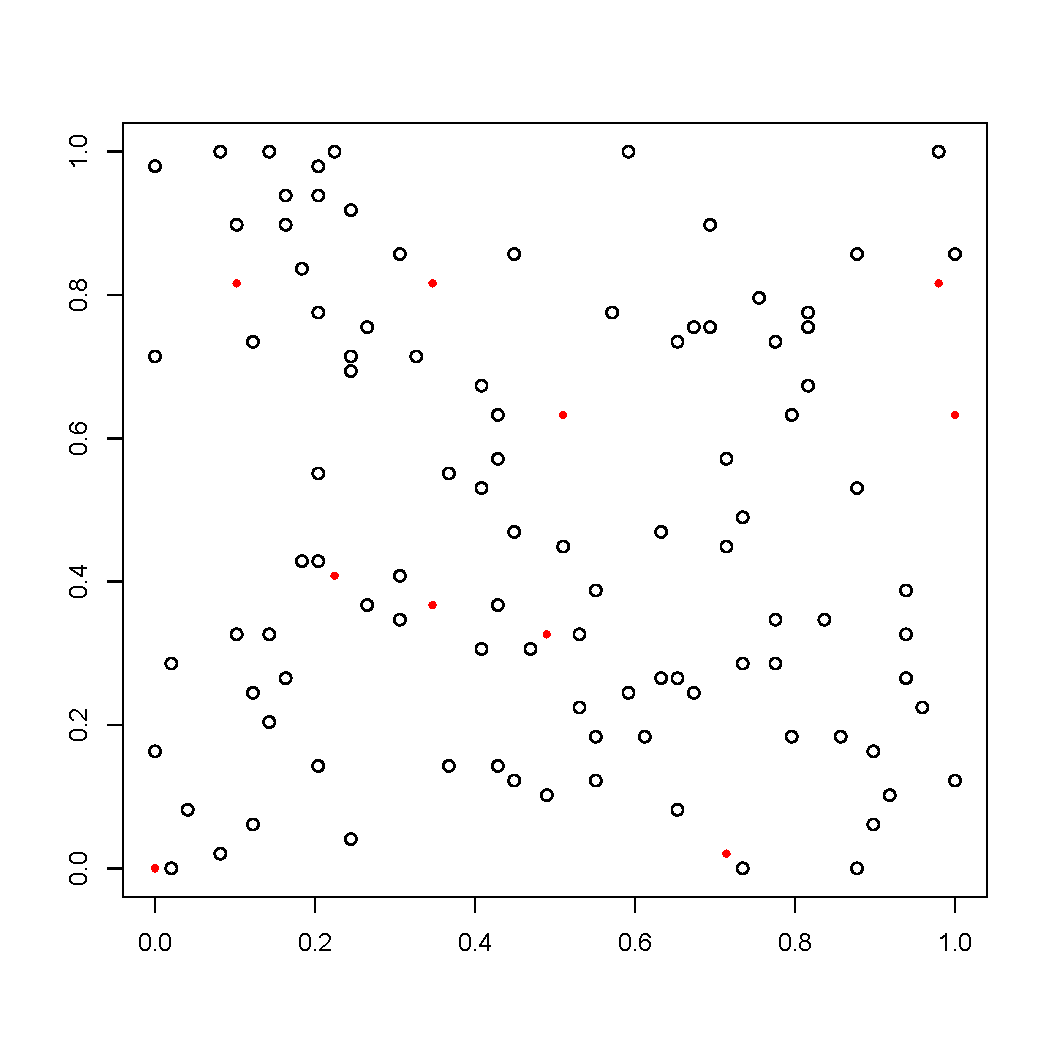
\includegraphics[width=0.5\textwidth]{images/kriging/locations.pdf}
\end{center}�
\caption{Locations of simulated curves. Solid dots are prediction locations.}
\label{fig:locations}
\end{figure}�

\begin{figure}
\begin{center}
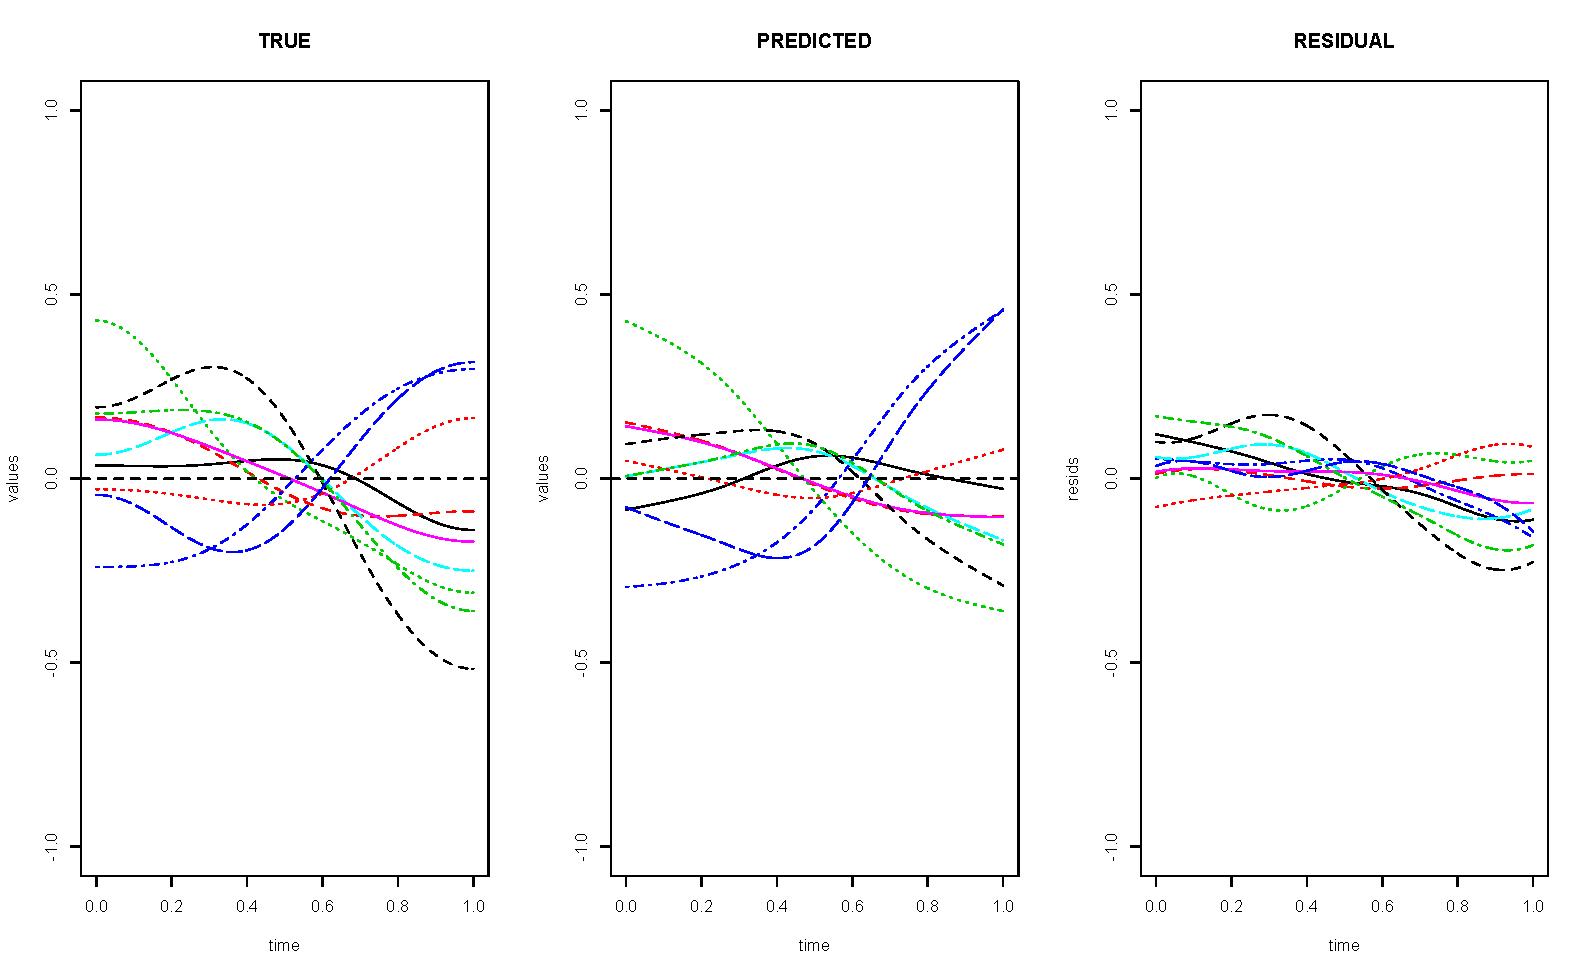
\includegraphics[width=0.6\textwidth]{images/kriging/residual-curves.pdf}
\end{center}�
\caption{Predicted curves at unobserved locations. }
\label{fig:curve kriging predictions}
\end{figure}�

%\subsection{Application}
%
%Include a application to real data. We have recently received a data set on forest canopy cover that could be a very interesting data set. 
\newpage
\subsection{Future Work}

The future work we would like to accomplish for this chapter consists of gaining a better understanding of how the covariance function estimator performs when the independence assumption is violated, and to explore possible modifications to both the covariance function estimator and smoothing parameter selection which account for spatial dependence. 

\subsubsection{Simulation framework useful for studying spatial dependence between curves}
By using the simulation framework in Chapter \ref{ch:covariance estimation}, but using a spatially correlated Gaussian random variables instead of uniform random variables we can investigate the effects of spatial dependence on estimation of functional principal components. Already included here is a simulated example under independence. 

Random curves are simulated independently as
\begin{equation}
X(t) = \sum^{3}_{k=1}\zeta_k Z_k \cos(k\pi t), \hspace{0.5cm} t \in [0,1],
\label{eq:sim process2}
\end{equation}�
where $Z_k$ were independently sampled from a $N(0,1)$ distribution and \(\zeta=(-1)^{k+1}k^{-\alpha}\). 
The covariance function for this process can be easily show to be
\begin{equation}
C(s,t) = \sum^{3}_{k=1}k^{-2\alpha} \cos(k\pi s)\cos(k\pi t). 
\end{equation}�

Figure \ref{fig:sim curves2} shows 100 curves simulated independently from the process in \eqref{eq:sim process} with $\alpha=2$. 


\begin{figure}
\begin{center}
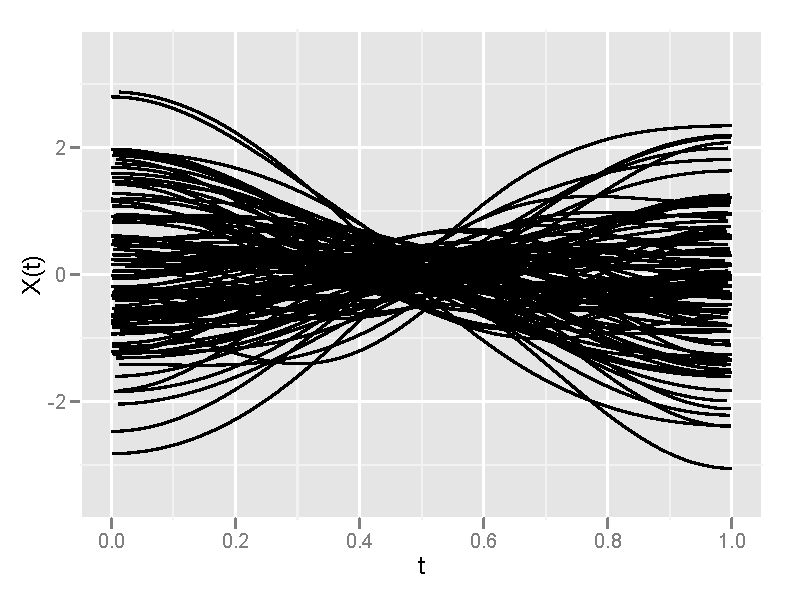
\includegraphics[width=0.5\textwidth]{images/Ch3/sim-curves.pdf}
\end{center}
\caption{One hundred curves simulated independently from the process $X(t)$ in \eqref{eq:sim process2}.}
\label{fig:sim curves2}
\end{figure}�


\begin{figure}
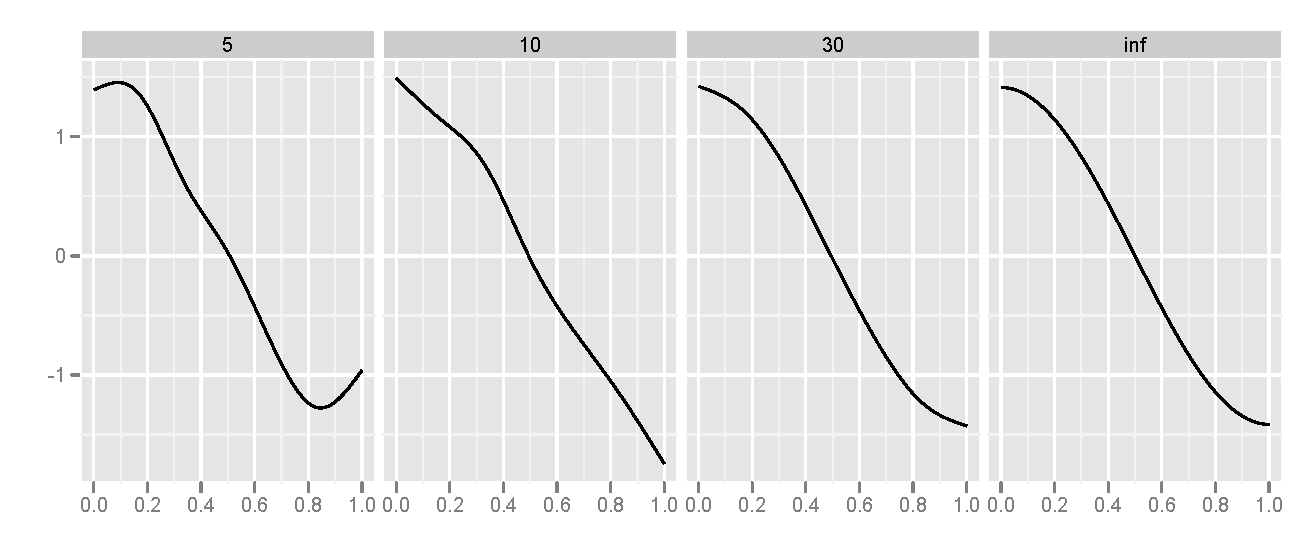
\includegraphics[width=\textwidth]{images/Ch3/eigenfun1-sig-0368.pdf}
\caption{1st eigenfunction estimated from 100 simulated curves, where each curves is observed at $m$ random locations with noise ($\sigma = 0.0368$). The number of observations per curve is indicated in the plot label. }
\end{figure}�

\begin{figure}
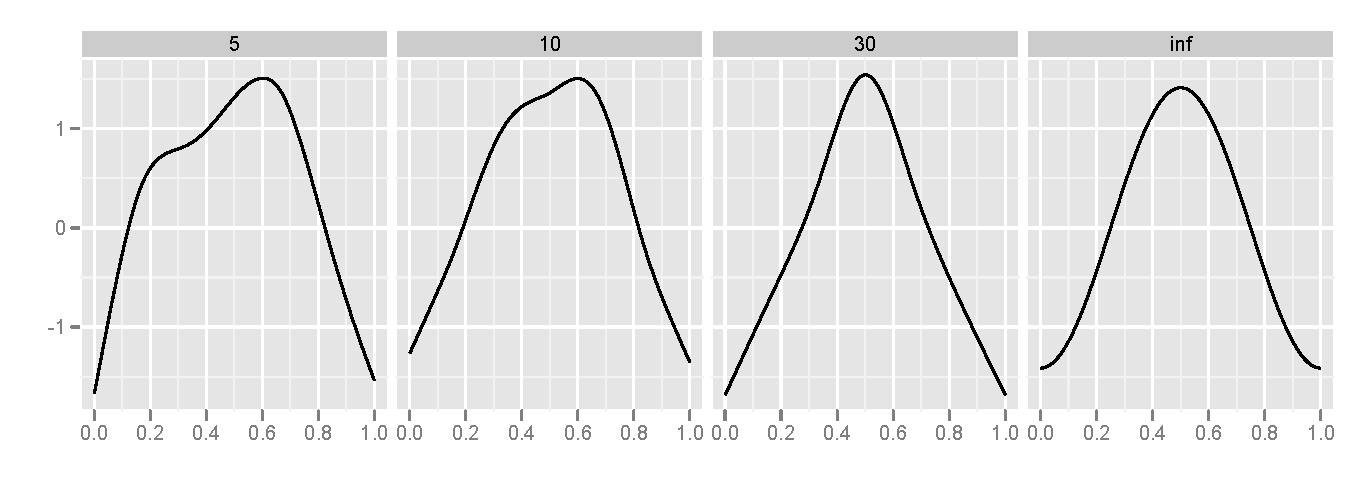
\includegraphics[width=\textwidth]{images/Ch3/eigenfun2-sig-0368.pdf}
\caption{2nd eigenfunction estimated from 100 simulated curves, where each curves is observed at $m$ random locations with noise ($\sigma = 0.0368$). The number of observations per curve is indicated in the plot label. }
\end{figure}�

\newpage
\subsubsection{Adjustments to the covariance function estimation which account for spatial dependence}

Let $\mathbf{b}^{(i)} = [(y_{ij}-\mu(t_{ij}))(y_{ij'}-\mu(t_{ij'}))]_{1\leq j\neq j'\leq m}$, $i=1, \dots, n$. Let
\[
\mathbf{b} = (\mathbf{b}^{(1)T}, \mathbf{b}^{(2)T}, \dots, \mathbf{b}^{(n)T}   )^T,
\]
then the vectors $\mathbf{b}^{(i)}$ contain values related to the sample covariance from curve $i$, and the vector $\mathbf{b}$ contains all sample covariance terms. 
 	The elements of $\mathbf{b}$ have non-trivial covariances due to spatial correlation among curves. However, we show that the elements of Cov$(\mathbf{b})$ can be compute using only covariances of the form \eqref{eq:cov}. Let
\[
\mathbf{W}= \text{Cov}(\mathbf{b}), 
\]

then elements of $\mathbf{W}$ can be computed as follows,
\begin{align} 
	\text{Cov}(\epsilon(s_i; t_{j}) \epsilon(s_i;t_{j'}), \epsilon(s_{i'}; t_{l}) \epsilon(s_{i'};t_{l'}) ) 
	&= 
	  \text{Cov}(\epsilon(s_i; t_{j}), \epsilon(s_{i'}; t_{l}))\text{Cov}( \epsilon(s_i;t_{j'}), \epsilon(s_{i'};t_{l'})  ) \nonumber \\
	&+
		 \text{Cov}(\epsilon(s_i; t_{j}),  \epsilon(s_{i'};t_{l'}) )\text{Cov}(\epsilon(s_i;t_{j'}), \epsilon(s_{i'}; t_{l})) \label{eq:cov of products}
\end{align}
The right hand side of \eqref{eq:cov of products} holds under the assumption of Gaussian distributions (see \cite{Bohrnstedt:2010ud}). 

We propose the following estimator
\[
\widehat{C}_{\lambda}=\stackrel[C \in \H\otimes \H]{}{\text{ argmin}} \left\{ l_{n}(C)+\lambda\left\Vert C\right\Vert _{\breve{\H}}^{2} \right\},
\]
 where

\begin{equation}
l_{n}(C)= (\mathbf{b} - \mathbf{C})^T\mathbf{W}^{-1}(\mathbf{b} - \mathbf{C})
\label{eq:weighted loss function}
\end{equation}
and 
\[
\mathbf{C} = [C(t_{i,j}, t_{i'j'})]
\]

%=====================================

\begin{itemize}
\item Though computation of $\mathbf{W}^{-1}$ is theoretically possible, the dimension of $\mathbf{W}$ is computationally prohibitive. To complete this chapter we intend to investigate the possibility of including weights in the loss function used in covariance function estimation (this would correspond to a diagonal $\mathbf{W}$ matrix in \eqref{eq:weighted loss function} ). If we think of the locations of the curves as a point process, then we can use the intensity function to derive weights for the curves.  A possible way to define appropriate weights would be the inverse intensity raised to some power. We intend on investigating appropriate choices through a simulation study, with the hope of being able to offer general guidelines for  choosing a weight function. We also intend on including weight function in the smoothing parameter selection. 
\end{itemize}
%\end{spacing}
%\todo[inline]{discuss how possible measures of interest (e.g. min, max, average) are functionals of the curve predictor. Should this go in the introduction? }

